\documentclass[12pt]{article}

\usepackage{xeCJK}%字體設定
\setCJKmainfont{cwTeXKai}[AutoFakeBold=1.5]


\setmainfont{Times New Roman}  % 英文正文字體

\usepackage[top=2cm,bottom=2cm,left=2cm,right=2cm,a4paper]{geometry}%版面設定

\usepackage{indentfirst}%縮排

\usepackage{setspace}%行距設計
\onehalfspacing%半行距
\setlength{\parskip}{3pt}%段落之間

\usepackage{moresize}%字體大小

\usepackage{graphicx}

\usepackage{amssymb}%數學符號

\usepackage{amsmath} % 數學符號
\usepackage{booktabs}         % 漂亮的表格（\toprule, \midrule, \bottomrule）
\usepackage{siunitx}          % 國際單位制 (建議處理單位更漂亮)

\usepackage{multicol}%引入函數使下面那些可以變成雙欄

\usepackage{float}%圖片固定
\usepackage{cite}

% \renewcommand{\thesection}{\Roman{section}}


%%%%%%%%%%%%%%%%%%%%%%%%%%%%%%正文%%%%%%%%%%%%%%%%%%%%%%%%%%%%%%%%%%%
\begin{document}

\begin{titlepage}
\begin{center}

\vspace*{0.5cm}
\HUGE \textbf{普通物理實驗結報}\\
\vspace{2cm}
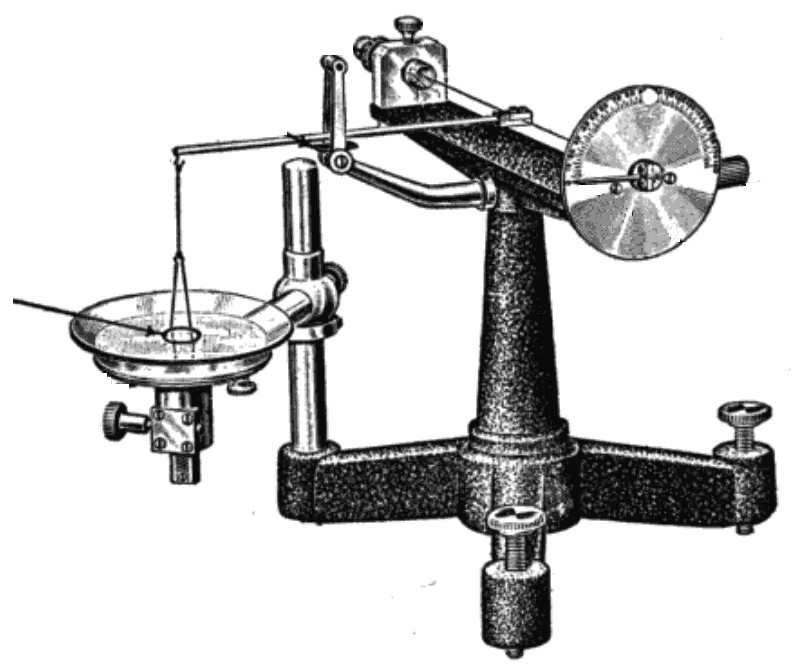
\includegraphics[width=13cm]{p.jpg}\\[2cm]
\HUGE \textbf{表面張力}\\

\vfill
\huge 第三組\\[0.5cm]
\begin{table}[h]
\centering
\Large
\begin{tabular}{|c|c|}
\hline
組員:              & 貢獻度  \\
吳& 37.5\% \\
卓& 37.5\% \\
程& 25\% \\ \hline
\end{tabular}
\end{table}

\end{center}

\end{titlepage}

%%%%%%%%%%%%%%%%%%%%%%%%%%%%%%%%%%%%%%%%%%%%%%%%%%%%%%%%%%%%%%%%

\large
\section{\textbf{實驗目的}}
To measure the \textbf{surface tension} of different types of liquids using a \textit{Du Noüy tensiometer}, and to observe how \textbf{different liquids }exhibit distinct responses and measured values of surface tension. 

%%%%%%%%%%%%%%%%%%%%%%%%%%%%%%%%%%%%%%%%%%%%%%%%%%%%%%%%%%%%%%%%

\section{\textbf{實驗原理}}
\textbf{Surface tension} is a property that describes a liquid’s tendency to \textit{minimize its surface area}. It arises from the \textbf{unbalanced molecular forces} experienced by molecules at the surface of the liquid. Molecules within the bulk of the liquid are surrounded by other molecules on all sides and thus experience balanced intermolecular forces, whereas\textit{ surface molecules lack neighbors on one side}, resulting in a net inward force that minimizes the surface area. 

\vspace{0.3cm}
\begin{figure}[H]
    \centering
    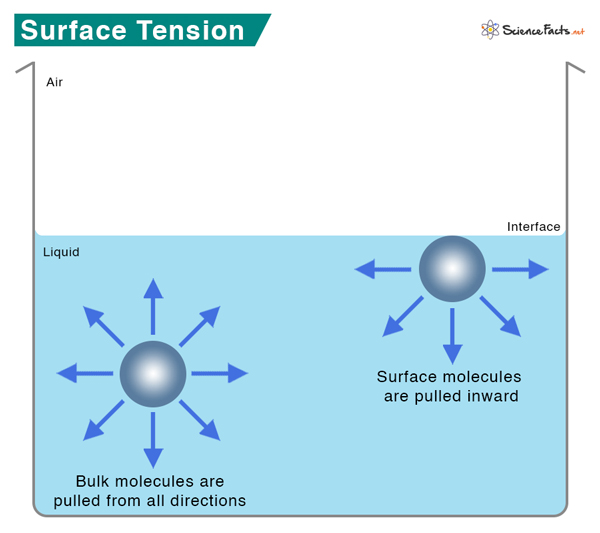
\includegraphics[width=0.35\linewidth]{Surface-Tension.jpg}
    \caption{Force diagram experienced by a molecule.}
    \label{fig:placeholder}
\end{figure}
In mathematical form, it can be written as:
\[\sigma=\Delta W/\Delta A\]
{\small
Surface tension is the \textit{ratio} of the energy required $\Delta W$ to increase a liquid’s surface area by a given amount $\Delta A$. In simpler terms, it measures \textbf{how much energy is needed to increase the surface area of a liquid}.
}

\vspace{0.3cm}
Another way to understand \textit{s}\textit{urface tension} is to consider a thin rod or ring partially submerged in a liquid. When the rod or ring is pulled upward, the liquid surface resists being stretched, exerting a \textbf{restoring force along the contact line}. In this scenario, the total force required to lift the object is \textit{proportional} to the length of the\textit{ contact line}. 

\begin{figure}
    \centering
    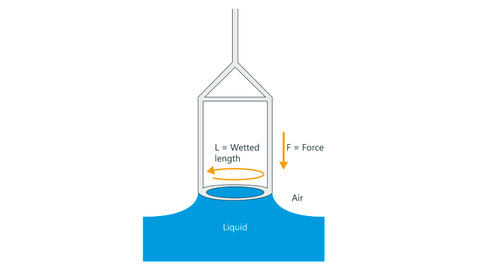
\includegraphics[width=0.8\linewidth]{kruss-glossary-tensiometer.83c69557.png}
    \caption{A Du Nouy tensiometer.}
    \label{fig:placeholder}
\end{figure}

\vspace*{0.5cm}
\hrule
\vspace*{0.3cm}
\[F=2\lambda T \ \ \textit{or} \ \ T=F/2\lambda\]
\noindent
which gives the working equation of \textbf{the Du Nouy tensiometer.}

\vspace{0.3cm}
{\small
Note:
\begin{itemize}
\item \textit{F} is the \textit{force used. ($dyne$)}
\item $\lambda$ is \textit{length of the contact line. ($cm$)}
\item \textit{T} is the \textit{surface tension} of the liquid. ($J/m^2$ or $dyne/m$)
\end{itemize}
}
\vspace*{0.3cm}
\hrule
\vspace*{0.3cm}
\subsection{\textbf{Reaction under Temperature}}

In chemistry, \textbf{temperature} is a measure of how energetically excited the molecules in a \textit{substance} are, which is directly related to their \textit{average kinetic energy}. As temperature increases, molecules move faster and vibrate more strongly. This increased motion reduces the amount of time molecules spend interacting with their neighbors, thereby weakening \textbf{cohesive forces} between them. Since \textit{surface tension }arises from these cohesive i\textit{ntermolecular force}s, a decrease in \textbf{cohesion} leads to a corresponding decrease in \textbf{surface tension.}

\vspace{0.3cm}
As shown in \textbf{Figure 3}, cohesive forces between molecules are responsible for a liquid droplet forming a\textit{ spherical shape.} Molecules located at the surface of the droplet experience \textbf{unbalanced} \textbf{intermolecular} \textbf{forces}, since they are not surrounded by neighboring molecules on all sides. This imbalance creates a net inward force that causes the surface to contract, effectively “tucking” the droplet inward and giving it its characteristic rounded shape.

\vspace{0.3cm}
The degree to which a droplet \textit{remains spherical }depends on the relative strength of these \textit{cohesive forces} compared to \textit{gravitational} \textit{forces}. If the cohesive forces are insufficient to overcome gravity, the droplet spreads out and appears \textbf{flatter}. For example, alcohol has weaker intermolecular (cohesive) forces than water, so its droplets tend to \textit{flatten} more readily, indicating a\textbf{ lower surface tensio}n. Conversely, certain solutes can increase surface tension. For instance, dissolved salts can enhance intermolecular interactions by forming \textit{stable hydration shells }around ions, which strengthens the overall \textbf{cohesion} between water molecules.

\subsection{Du Nouy Tensiometer}
As a note, the \textbf{Du Nouy tensiometer} uses a metal ring to measure surface tension, as shown in Figure 2. The ring provides a \textbf{stable and well-defined perimeter}, which is required for applying the surface tension formula, and it also acts as a frame on which a thin liquid film can form. As an upward force is gradually applied, the liquid film stretches until it eventually breaks. The force at the moment of detachment corresponds to the \textbf{maximum force sustained by the surface tension}, representing the strength of the liquid’s cohesive forces at the surface.
\[F_{max}=2\lambda T\]
%%%%%%%%%%%%%%%%%%%%%%%%%%%%%%%%%%%%%%%%%%%%%%%%%%%%%%%%%%%%%%
% \section{\textbf{理論分析}}

% 這裡放文字

%%%%%%%%%%%%%%%%%%%%%%%%%%%%%%%%%%%%%%%%%%%%%%%%%%%%%%%%%%%%%%%%
\newpage
\section{\textbf{實驗方法}}
\subsection{實驗一:修正張力計}
使用法碼校正張力計上的刻度。
\subsection{實驗二:水在不同溫度的表面張力}
加熱純水至不同的溫度，觀察其表面張力的變化。
\subsection{實驗三:測量不同溶液的表面張力}
分別測量，水、食鹽水、肥皂水之表面張力。
\subsection{實驗四:測量酒精在不同體積百分濃度的表面張力}
實驗步驟同實驗二、三。
%%%%%%%%%%%%%%%%%%%%%%%%%%%%%%%%%%%%%%%%%%%%%%
\section{\textbf{數據分析}}
%%%%%%%%%%%%%%%%%%%%%%%%%實驗一%%%%%%%%%%%%
\subsection{實驗一:校正表面張力儀器}
\begin{figure}[H]
    \centering
    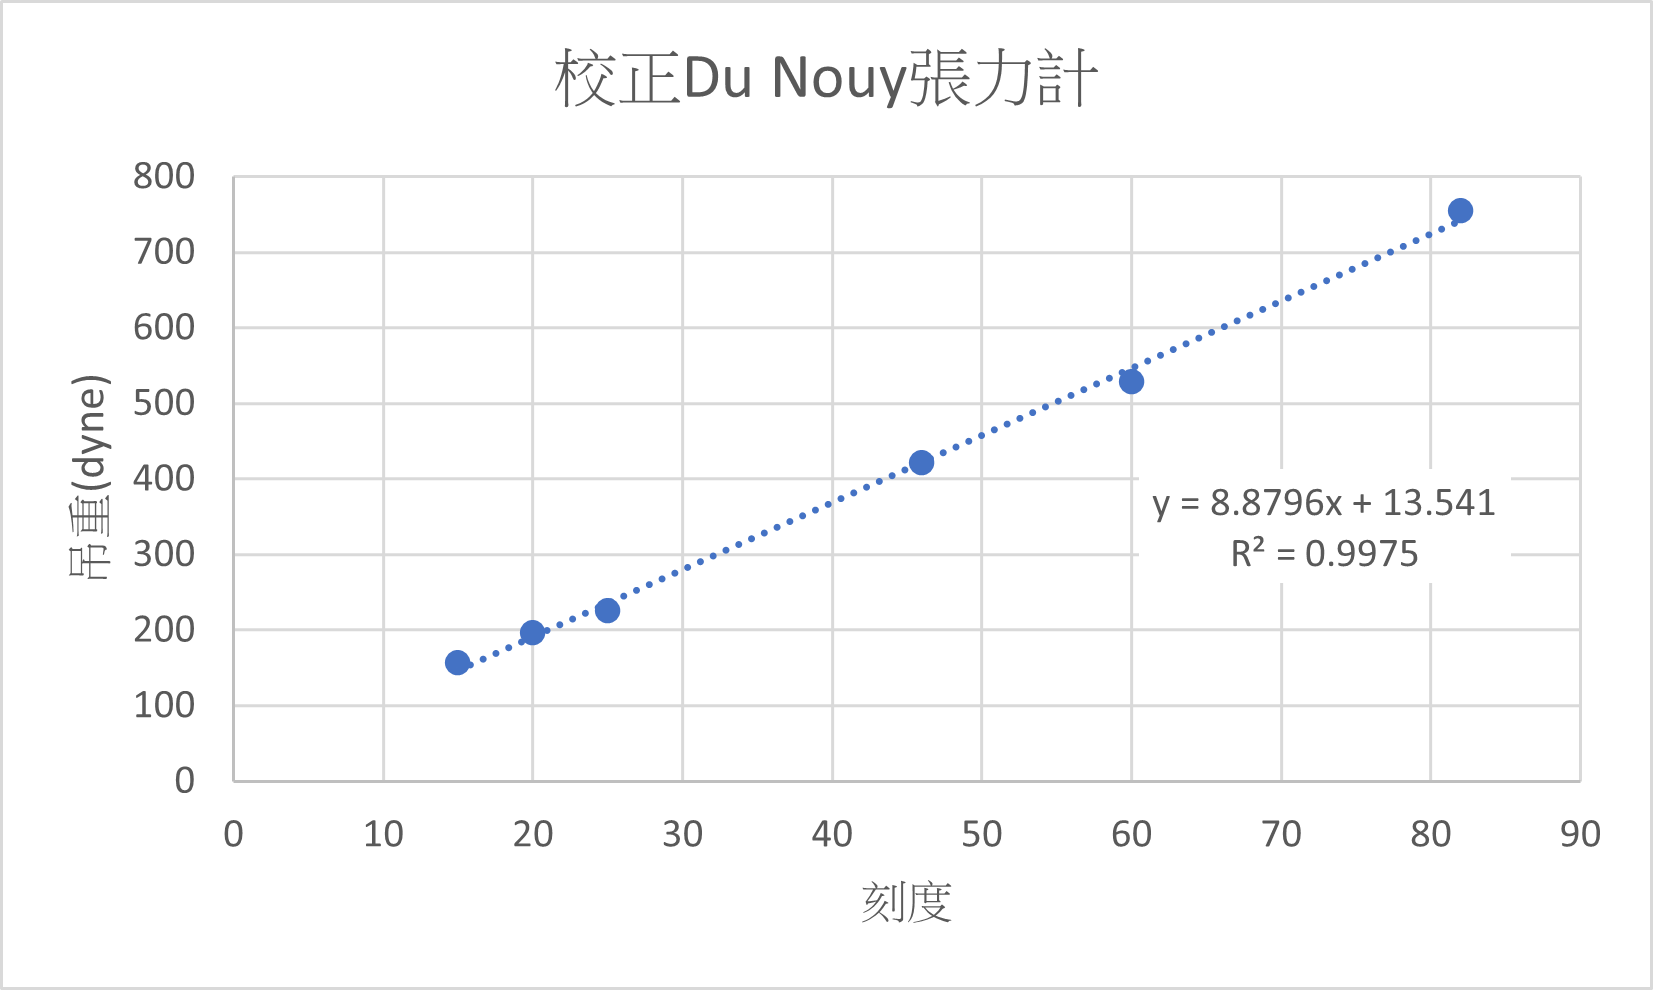
\includegraphics[width=0.7\linewidth]{圖表/校正儀器.png}
    \caption{儀器刻度與吊重關係圖}
    \label{fig:關係圖}
\end{figure}
因為在校正儀器時並未算入後續掛上的吊環，故在後續實驗計算中都將扣除45 dyne重之吊環。
%%%%%%%%%%%%%%%%%%%%%%%%%%%%%%實驗二%%%%%%%
\subsection{實驗二:水在不同溫度的表面張力}
\begin{figure}[H]
    \centering
    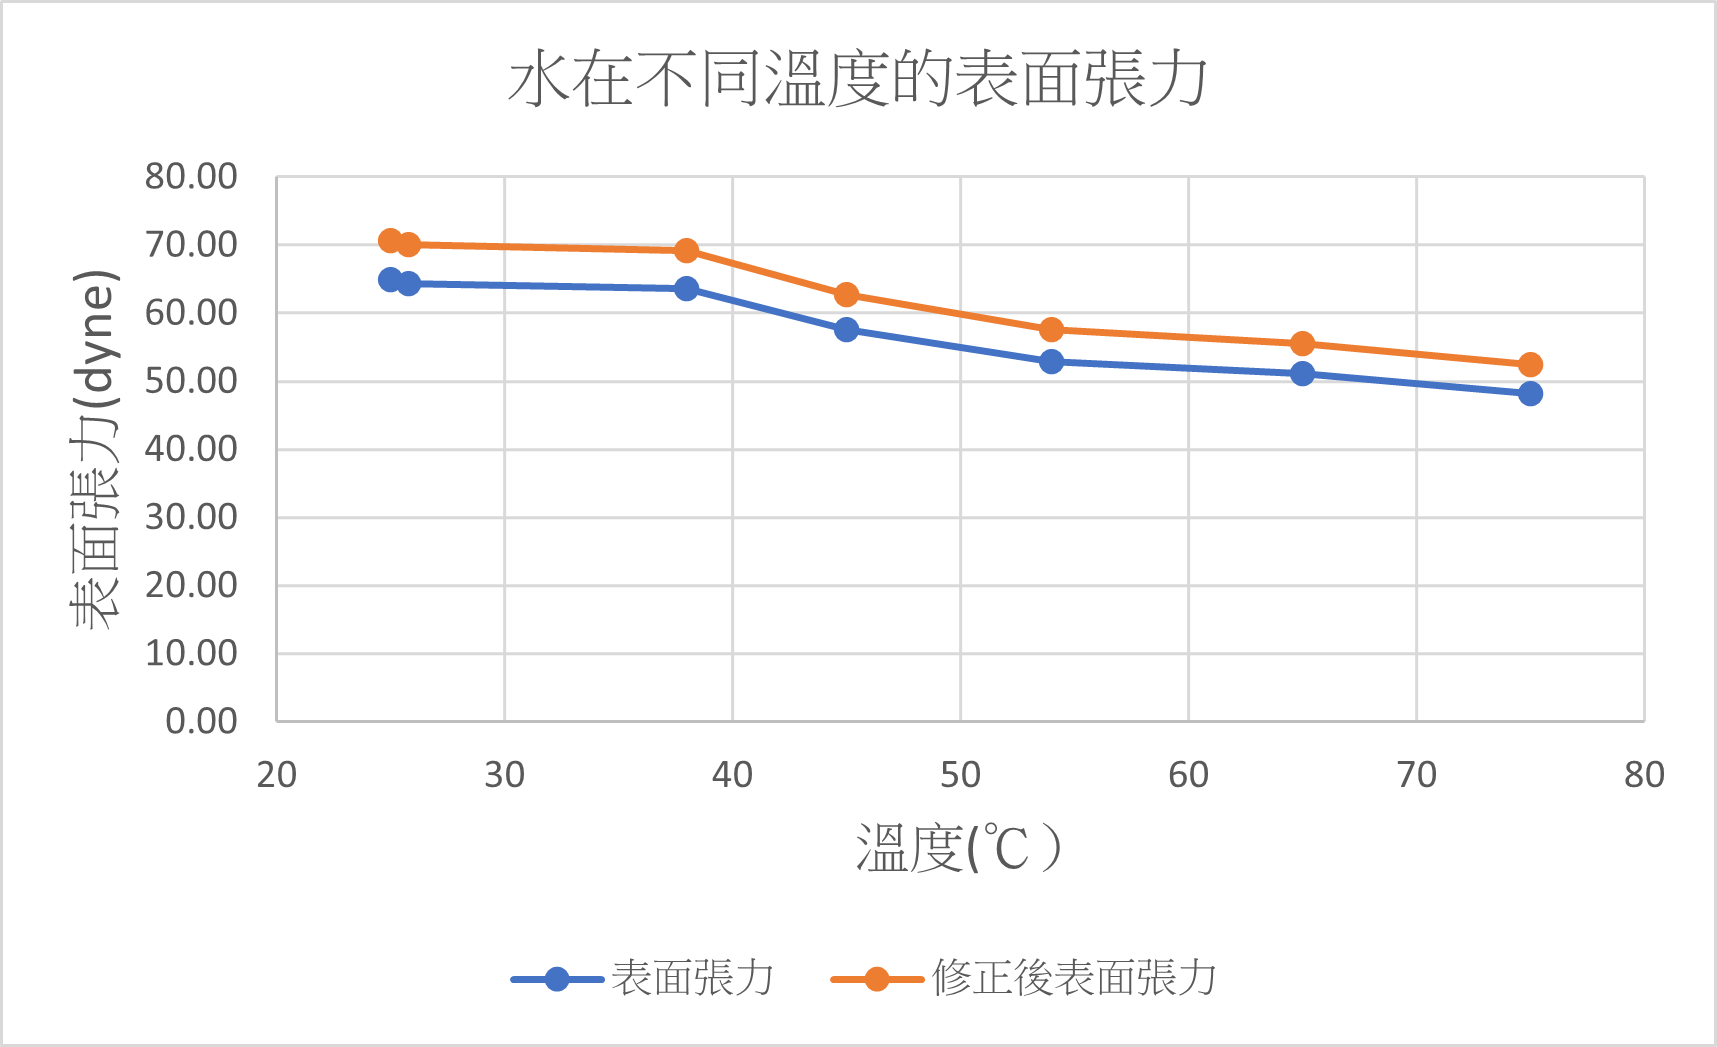
\includegraphics[width=0.7\linewidth]{圖表/水在不同溫度的表面張力.png}
    \caption{水溫與表面張力關係圖}
    \label{fig:placeholder}
\end{figure}
Du Noüy 環法中的修正係數源自 Harkins 與 Jordan \cite{HarkinsJordan1930}.對懸鍊面形狀進行的實驗與數值分析，其結果以查表形式給出。實務上，對於低 Bond number（如水、食鹽水、肥皂水）且常見的圓環條件，修正係數常以對原始表格數據的經驗公式近似表示，其主要依賴於環半徑與線半徑之比。
給出的修正係數經驗公式$f(\frac{R}{r},\frac{\rho gR^2}{\gamma})$中，水這種低密度的流體可近似成
\[
f(\frac{R}{r})=1-\frac{0.725}{\sqrt{R/r}}+\frac{0.0142}{R/r}
\]
實驗中測量到的環半徑(R)=10.8mm與線半徑(r)=0.3mm，計算可得張力計修正係數$f\approx 1.088$，故在後續實驗中會展示修正後得結果。
\[
T_{result}=T_{exp}\cdot f
\]
\newpage
誤差分析:
\begin{itemize}
    \item 將修正後的數據與講義資料做比較，發現在25-30度區間較相近，然而高溫區間就出現較大的差距。推測應是實驗中並不是以純水作為實驗溶液，而是用含有礦物質、氯離子的自來水，這些離子在獲得較多動能後，就更高頻的撞擊表面水分子，破壞表面水分子的緊密性，造成表面張力下降。
\end{itemize}
%%%%%%%%%%%%%%%%%%%%%%%%%%實驗三%%%%%%%%%%
%%%%%%%%%%%%%%%%%%%%%%%%%%%%%%%%%%%%%%%%%%%%%%
\subsection{實驗三:不溶液之表面張力}
\begin{figure}[H]
    \centering
    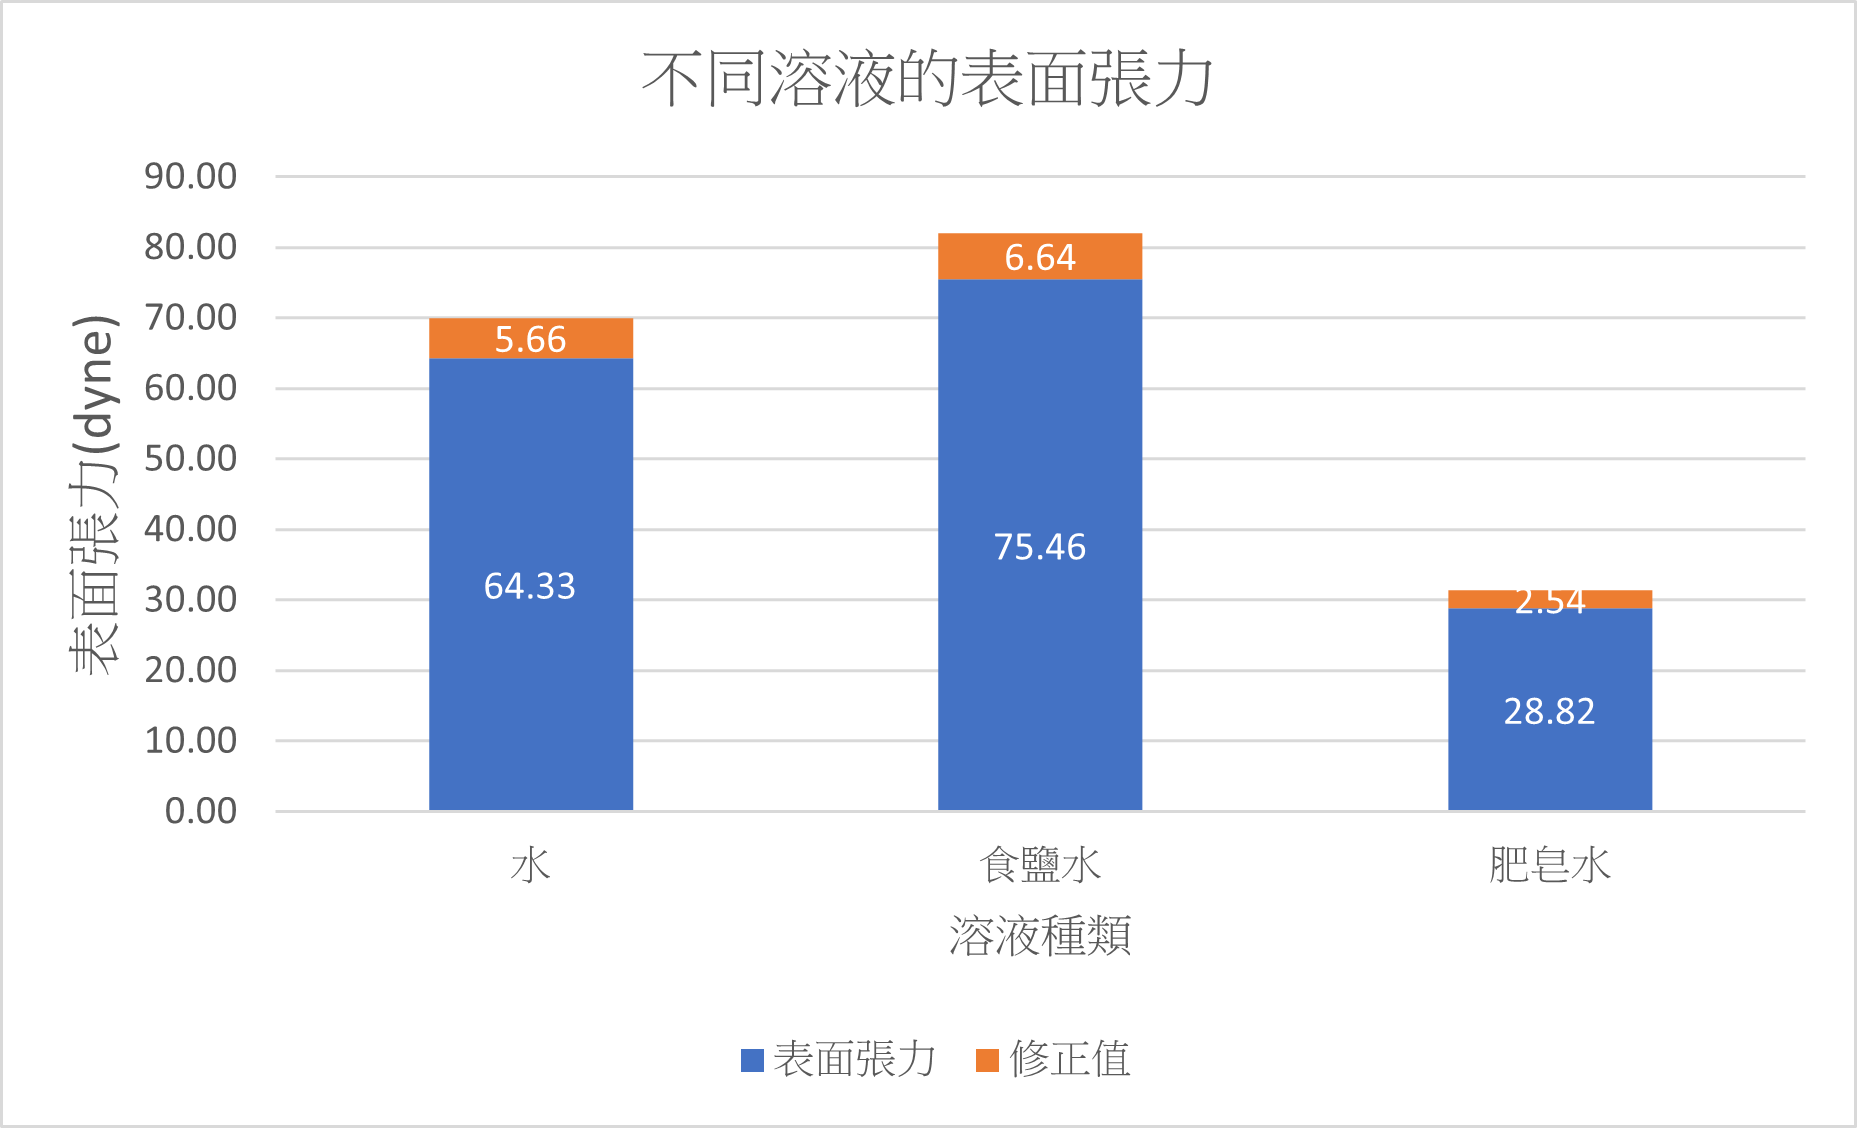
\includegraphics[width=0.7\linewidth]{圖表/不同溶液的表面張力.png}
    \caption{溶液的表面張力}
    \label{fig:placeholder}
\end{figure}
由數據可見，表面張力由大到小分別是，食鹽水>自來水>肥皂水，原因食鹽水中的$Na^+$與$Cl^-$吸引水分子，提供更大的內聚力，使表面張力增加;肥皂水則是因為界面活性劑在液面均勻排列，造成表面張力下降。\\



%%%%%%%%%%%%%%%%%%%%%%%%%%實驗四%%%%%%%%%%%
\subsection{體積百分濃度對酒精溶液表面張力之影響}
\begin{figure}[H]
    \centering
    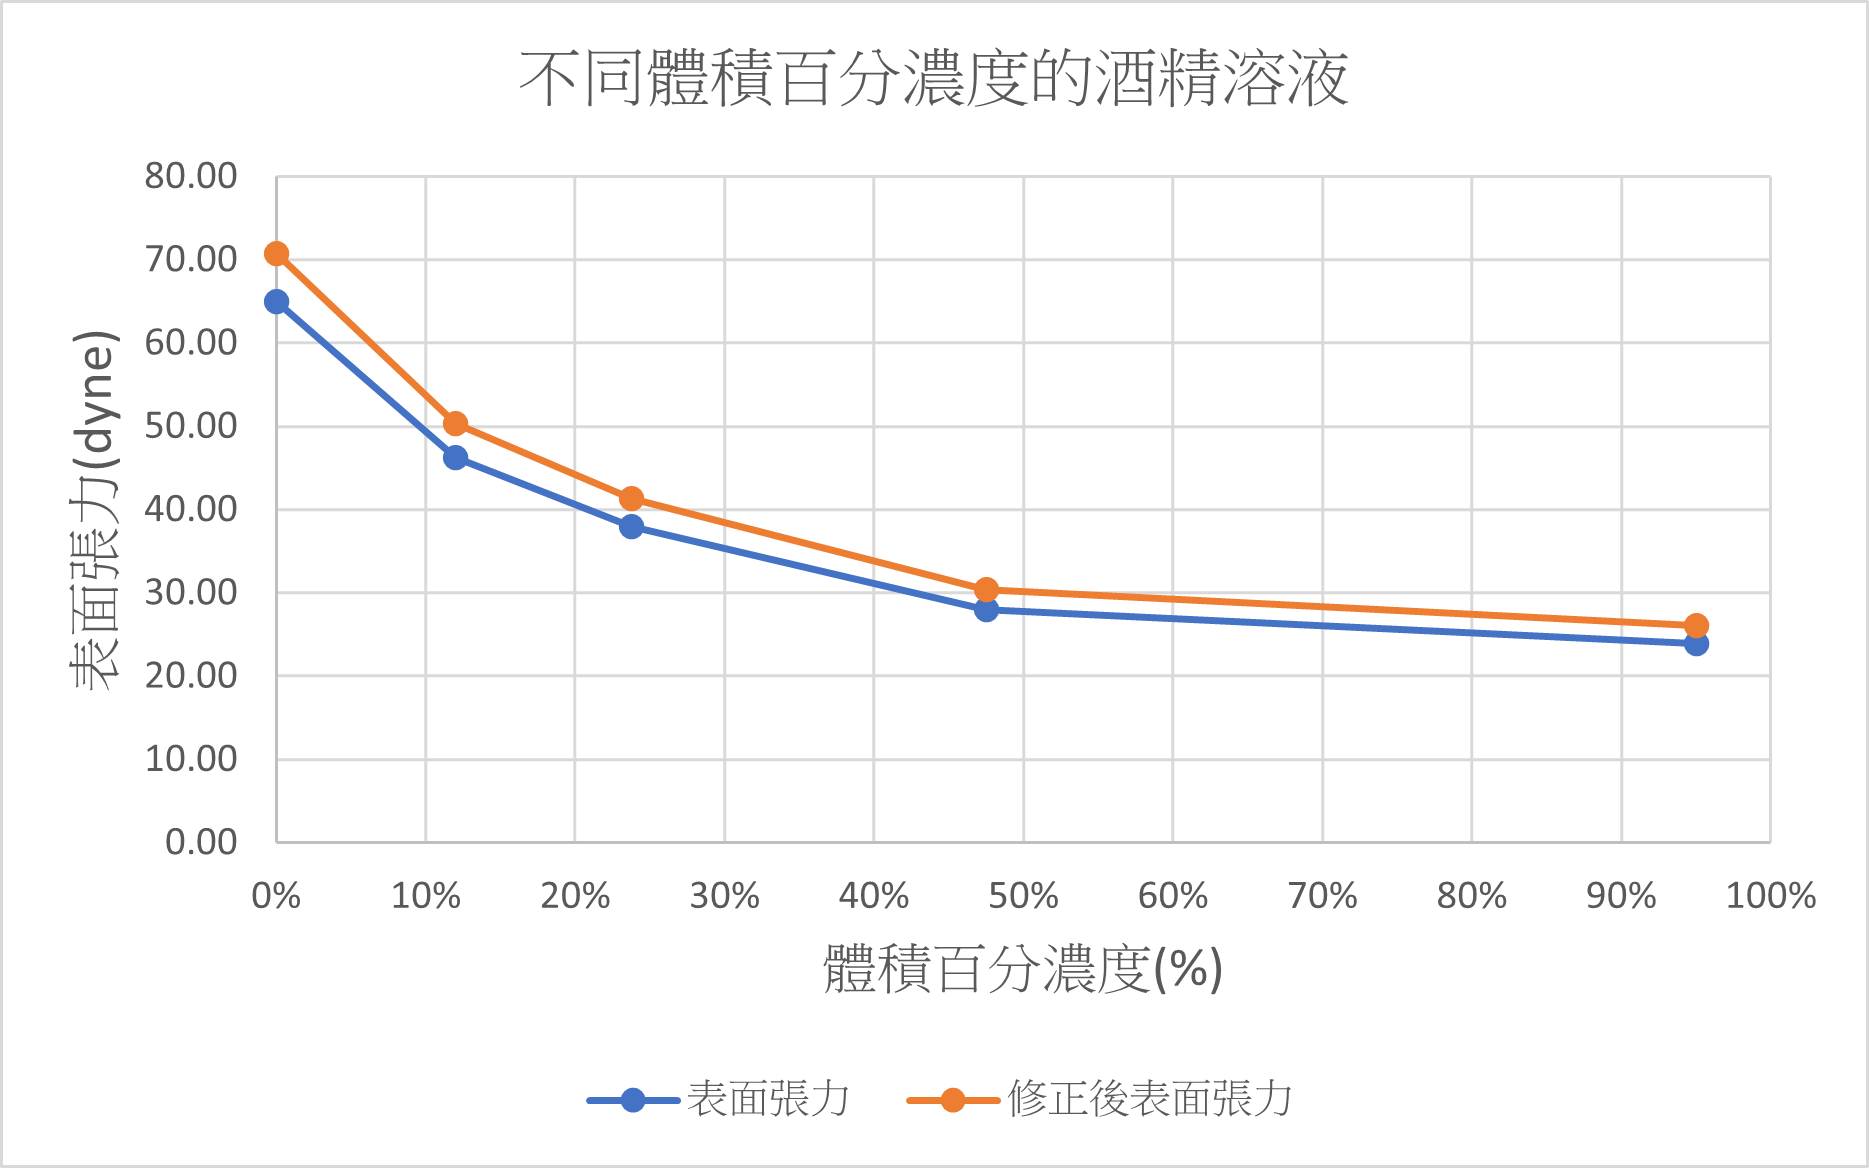
\includegraphics[width=0.7\linewidth]{圖表/不同體積百分濃度的酒精.png}
    \caption{不同體積百分濃度酒精的表面張力}
    \label{fig:placeholder}
\end{figure}
由實驗數據可見，酒精溶液隨著濃度增加，表面張力逐漸下降。原因如下：
\begin{itemize}
    \item 酒精分子比水分子較小且氫鍵能力弱，其內聚力低於水分子。
    \item 當酒精加入水中時，酒精分子會部分替代水分子在液面的位置，削弱液面的氫鍵。
    \item 濃度越高，液面氫鍵越少，表面張力下降越明顯。
\end{itemize}




%%%%%%%%%%%%%%%%%%%%%%%%%%%%%%%%%%%%%%%%%%%%%%%%%%%%%%%%%%%%%%%%
\newpage
\section{\textbf{結果與討論}}
本實驗透過 Du Noüy 環法成功量測了多種條件下的表面張力，並證實了表面張力與液體本質及溫度之密切關係。實驗數據顯示，水的表面張力隨溫度升高而呈現下降趨勢，主因在於分子動能增加削弱了分子間的內聚力；在溶液比較方面，食鹽離子透過離子-偶極力強化了液體內部的吸引力，而肥皂水與酒精則因界面活性劑排列或分子間作用力較弱，顯著降低了表面張力。此外，實驗過程中計算出的修正係數（$f \approx 1.088$）有效地補償了液膜受重力影響產生的形變，證明了在利用環法測量時，考慮幾何因子與系統偏差對於獲得準確物理量的重要性。

在誤差分析與精確度評估方面，本實驗量測值與文獻值之偏差主要源於材料純度與環境控制之限制。首先，實驗中使用含有礦物質離子的自來水而非純水，這些雜質在高溫下運動更趨劇烈，容易破壞表面水分子的緊密結構，導致高溫區間的數據偏差較理論值明顯。其次，操作時旋轉刻度盤的速度不均，以及液面與金屬環未能達到絕對水平，均會導致液膜斷裂時的張力產生跳動。未來實驗建議改用自動升降裝置以排除人為操作誤差，並使用$ddH_2O$進行實驗，以進一步提升測量精確度並降低系統誤差。
\newpage
\section{\textbf{思考問題}}
\begin{enumerate}
    \item \textbf{你的實驗結果準確度如何？試解釋可能的誤差來源。}

    \noindent
    實驗結果整體與文獻值相符，但存在一些誤差。可能的誤差來源包括：
    \begin{itemize}
        \item 使用自來水而非純水，水中的礦物質、離子會影響表面張力。
        \item 操作時液膜不完全水平或拉起過快，造成力的大小改變的誤差。
        \item 溫度控制不穩定。
    \end{itemize}

    \item \textbf{步驟 5 中列有兩種不同的歸零方法，哪一種可以得到比較準確的結果？為什麼？}
    \noindent
    \begin{itemize}
        \item 歸零方法若使用「無液體環狀測試」作為零點，會更準確，因為可以扣除環本身重量及張力計初始偏差。
    \end{itemize}

    \item \textbf{試比較代入(2)式與(4)式所求出的表面張力，哪一個可得到比較準確的結果？為什麼？}
    \noindent
    \\
    式4會較精準，因為利用純水作為標準液，計算待測液體的相對表面張力，可抵消環重與系統偏差，因此更準確。
    
    \item \textbf{加入少量的鹽，會稍微改變水的表面張力，若加入少量的油，則表面張力會有很大的改變，為什麼？試解釋之。}

    \noindent
    \begin{itemize}
        \item 鹽離子增加水中氫鍵，僅微幅提升表面張力。
        \item 油為非極性分子，破壞水分子間氫鍵，並形成液面薄層，顯著降低表面張力。
        \item 因此油對表面張力影響遠大於鹽。
    \end{itemize}

    \item \textbf{較冷的湯，油會均勻地分布在湯表面；而高溫時，油在湯表面的分佈變得不均勻，一團一團的，試解釋其原因。}

    \noindent
    \begin{itemize}
        \item 冷湯：表面張力高且油黏度較高，油滴擴散慢但穩定，分布均勻。
        \item 高溫湯：表面張力降低，油黏度下降，油滴容易聚合或快速漂浮，形成不均勻的油團。
        \item 此現象可用表面張力與溫度、油黏度的關係解釋。    
    \end{itemize}

\end{enumerate}
%%%%%%%%%%%%%%%%%%%%%%%%%%%%%%%%%%%%%%%%%%%%%%%%%%%%%%%%%%%%%


\noindent

\renewcommand{\refname}{參考文獻}
\bibliographystyle{unsrt}
\bibliography{參考文獻}
\end{document}